\documentclass[../main.tex]{subfiles}
\begin{document}
\setchapterstyle{kao}
\setchapterpreamble[u]{\margintoc}
\chapter[The exponential map of $G$]{The exponential map of $G$\footnotemark[0]}
\labch{exp-map-g}
The title may seem a mistake, because we already discussed the exponential map, but the emphasis is on the last two words: "\textit{of $G$}", where $G$ is a Lie group. 
\section{Definition and main theorem}
We already know, for every $X\in\textrm{Mat}(n,\mathbb{C})$, who is the exponential of $X$, namely $e^X=\sum_{n=0}^{+\infty}\frac{1}{n!}X^n$, and the same holds true for bounded operators in Hilbert spaces. But now there is a definition, which seems tautological: we take this map and we restrict it to $X$ in the Lie algebra of the Lie group $G$, and this is the exponential map of $G$.
\begin{definition}[Exponential map of a matrix Lie group]\index{Exponential map of a matrix Lie group}
Given a matrix Lie group $G$ with $\textrm{Lie}G=\mathfrak{g}$, the \textbf{exponential map of $\mathfrak{g}$} is the map which takes $X$ and sends it in the exponential of $X$, but regarded as a map from the Lie algebra to the Lie group:\marginnote{Of course if $X$ is in the Lie algebra, the exponential of $tX$ is in the Lie group for every $t$, and in particular for $t=1$. So if we start in the Lie algebra, we arrive in the Lie group, this is essentially by definition of matrix Lie algebra}
\[
\begin{split}
    \exp:\mathfrak{g}&\to G\\
    X&\mapsto e^{X}
\end{split}
\]
\end{definition}
Now we want to study the properties of this guy, so with the restriction that $X$ should be in the Lie algebra of $G$. We already know, from \vrefch{Matrix-Exponential-and-Logarithm}, that for every $A\in\textrm{GL}(n,\mathbb{C})$ there exists a matrix $X\in\textrm{Mat}(n,\mathbb{C})\equiv\mathfrak{gl}(n,\mathbb{C})$ such that {\color{red}$e^{X}=A$}.\marginnote[-5mm]{So if $G$ is the general linear group, then the exponential map is surjective.

From \cite{Hall2015_Ch3}: \textit{Nevertheless, if $G\subset \textrm{GL}(n;\mathbb{C})$ is a closed subgroup, there may exist $A$ in $G$ such that there is no $X$ \textbf{in the Lie algebra $\mathfrak{g}$} of $G$ with $\exp{X}=A$.} Therefore we think is more correct to say that, if $G<\textrm{GL}(n,\mathbb{C})$ \textbf{it is not \underline{ always} surjective.}

Actually is not even injective in some cases (see next page).}

{\color{red}{\fontencoding{U}\fontfamily{futs}\selectfont\char 66\relax} if $G<\textrm{GL}(n,\mathbb{C}$)} ("<" and not "$\leq$"!) the $\exp:\mathfrak{g}\to G$ is \textbf{not surjective!}
\begin{example}
Take $G=\textrm{SL}(2,\mathbb{C})$. We will convince ourselves that there is no $X\in\mathfrak{sl}(2,\mathbb{C})$ ($2\times 2$ complex matrices with zero trace) such that\marginnote[10mm]{We decide to call it $M$, where the letter stands for \textit{\textbf{M}atrix}}
\[
e^X=\mqty(-1 & 1 \\ 0 & -1)=M \in \textrm{SL}(2,\mathbb{C})
\]
This is an element of the special linear group because it is invertible (no eigenvalue zero) and the determinant is one, it is already in Jordan form. We are claiming that it is not the exponential of anything in the special linear algebra.

In fact, there are just two cases
\begin{enumerate}
    \item If $X$ has different eigenvalues, then it is \textbf{diagonalizable}, but then the exponential of $X$ will be (up to a similarity transformation)
    \[
    e^X=S\;\mqty(\dmat[0]{e^{\lambda_1}, e^{\lambda_2}})\;S^{-1}
    \]
    and it would be also diagonalizable, unlike $M$.
    \item If $X$ has coincident eigenvalues $\lambda_1=\lambda_2=0$ (since $\Tr{X}=0$). Then it means there is an eigenvector $v$ with eigenvalue zero, and when we apply $e^X$ to this eigenvalue 
    \[
    e^Xv=\sum\frac{1}{n!}X^nv=\left(1+\right)v
    \]
    then $e^X$ should have eigenvalue $1$, unlike $M$ (who has eigenvalue $-1,-1$).
\end{enumerate}
\end{example}
{\color{red}{\fontencoding{U}\fontfamily{futs}\selectfont\char 66\relax} In general, the map $\exp:\mathfrak{g}\to G$ is \textbf{not injective}.}
\begin{marginfigure}
	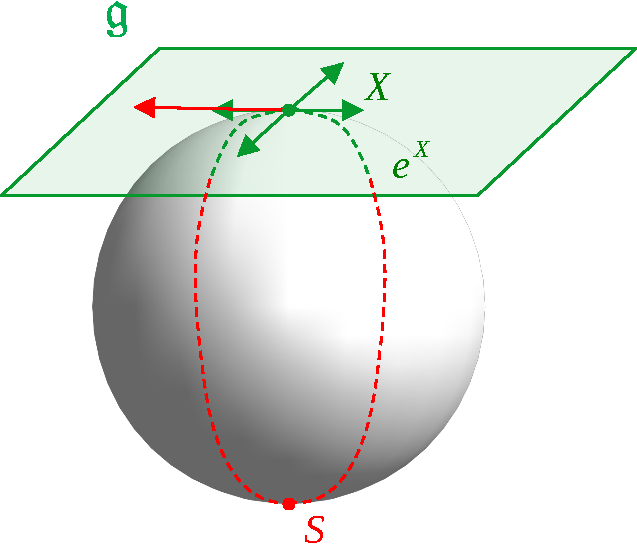
\includegraphics[width=1.2\linewidth]{images/su2_not_inj.pdf}
	\caption{$\textrm{SU}(2)$ non injective sphere.}
	\labfig{su2_not_inj}
\end{marginfigure}
\begin{example}
The simplest example is $\textrm{SU}(2)\simeq S^3$ (topologically is the three dimensional sphere): choose coordinates in such a way that the identity is at the North pole (we can always do that). If we take a tangent vector at the North pole, the exponential of $tX$ (where $X$ is the tangent vector) will be geometrically a meridian in our sphere and it will define a geodesic as far $X$ is short (dotted lines). So, we will have injectivity as far as our time is small: a small neighboured of the North pole will be diffeomorphic to a disk in the tangent plane to the North pole. But with a long time $t$, the meridians will collide each other to the South pole, so the map will not be injective. This happens, more in general, for $\textrm{SU}(n)$.

(This is not completely worked out, we are using the fact that the exponential of $tX$ is also the geodesic on the sphere, which we did not discuss in this \textit{Dispense}, with respect to a natural \href{https://en.wikipedia.org/wiki/Riemannian_geometry}{Riemmanian geometry.})
\end{example}
{\color{red}\raisebox{-\mydepth}{{
\includegraphics[height=1.1\baselineskip]{images/smile.jpg}}}\underline{Good news!}} The exponential map $\mathfrak{g}\xrightarrow{\exp}G$ is \textbf{locally bijective!}

The fact that the pathology we mentioned happens far away from the identity has to do with the fact that the logarithm and the exponential has the inverse to each other if we are close to zero, or respectively to one/identity, in a proper sense. Recall that it $\exists$ a magic number $\varepsilon_0: \quad \text{if} \norm{X}<\varepsilon_0 \ \Rightarrow \ \log(e^X)=X$. For $\norm{\dots}=\norm{\dots}_{\textrm{HS}}$ then $\varepsilon_0=\log(2)$

\underline{Visualization}: Take the linear space of $n\times n$ complex matrices, it has (real) dimension $2n^2$. In this linear space we define a neighbourhood (an open set) of zero called $\pazocal{V}_\varepsilon$:
\[
\textrm{Mat}(n,\mathbb{C})\supseteq \pazocal{V}_\varepsilon
\]
as represented in \reffig{vis-exp-G}. In a sense, this set will be small because its radius (so-to-speak) will be of order $\varepsilon$, so its diameter will be order $2\varepsilon$
\begin{figure}[h!]
	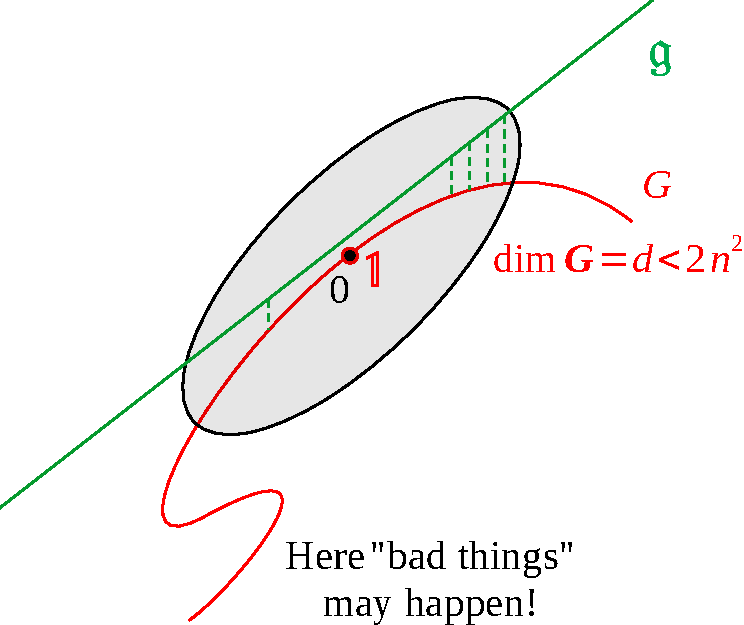
\includegraphics[width=1\linewidth]{images/visualization_exp_G.pdf}
	\caption[Visualization of the exponential map of $G$]{Diameter is well-defined even if we have something which is not a ball: it is the supremum over the distances between pair of points.}
	\labfig{vis-exp-G}
\end{figure}. But on the other hand, this set will be large, in the sense that its dimension is large: 
\[
\dim \pazocal{V}_\varepsilon=2n^2
\]
Now we have to double our picture, since the distinguish point in the Lie group is the identity, while the distinguish point in the algebra is zero. We overlap the pictures, imagining to have two copies of this linear space, and we shift them in such a way that the identity in red is exactly below the zero in black. The group is large in the sense of the diameter, but it has a small dimension $\dim G=d<2n^2$. The Lie algebra $\mathfrak{g}$ will be the tangent to the group, but tangent with the same dimension: it will be a linear subspace of the full space of matrices. Our theorem will tell us that if we are inside the neighbourhood, the exponential map is one-to-one, while if we are far away, bad things might happen (lack of injectivity, lack of surjectivity).
\begin{theorem}\labthm{main-exp-map}
For every $0<\varepsilon<\log(2)$, define \marginnote{So $\pazocal{V}_\varepsilon$ is not a ball in the strict sense, but topologically is still a ball (since the exponential is smooth, so it is the image of a ball via the exponential map).}
\[
\begin{split}
\pazocal{U}_\varepsilon&=\Bqty{X:\norm{X}<\varepsilon}\\
\pazocal{V}_\varepsilon&=\exp(\pazocal{U}_\varepsilon)
\end{split}
\]
Therefore there $\exists\;\varepsilon\in\left(0,\;\log(2)\right)$ such that, for every $A\in \pazocal{V}_\varepsilon$, it happens that\marginnote{Which means, if we rephrase it, that there is a one-to-one correspondence between Lie algebra and Lie group.}
\[
\log(A)\in\mathfrak{g} \ \Leftrightarrow \ A\in G
\]
\end{theorem}
\begin{proof}
Omitted (it is not difficult, but it is long, you can see it in \sidecite{Hall2015_Ch3})
\end{proof}
\subsection{Corollaries}
\todo{Hp: $G$ is a matrix Lie group, $\textrm{Lie}G=\mathfrak{g}$}
\begin{corollary}
There exists a neighbourhood $U$ of $\;0\in\mathfrak{g}$ and a neighbourhood $V$ of $\;\mathbb{1}\in G$ such that
\[
\exp\big|_U:U\to V
\]
is a \textbf{diffeomorphism}\marginnote[-10mm]{
With "neighbourhood $U$ of $\;0\in\mathfrak{g}$", we mean something which has the same dimension of $\mathfrak{}{G}$. 

It is a local diffeomorphism.

In this course in $C^\infty$-smooth, even tough in analysis it was $C^1$-smooth}, i.e. $C^\infty\textrm{-smooth}$ bijection with $C^\infty$-smooth inverse
\end{corollary}
\begin{proof}
\underline{Sketch of proof}: From the main \refthm{main-exp-map}, define
\[
\begin{split}
    U&=\pazocal{U}_\varepsilon\cap\mathfrak{g}\\
    V&=\pazocal{V}_\varepsilon\cap G
\end{split}
\]
and check that $\exp\big|_U:U\to V$ is a bijection. Then it remans to check that it is a $C^\infty$-smooth (that it is a diffeomorphism).
\end{proof}
\begin{marginfigure}[-10mm]
	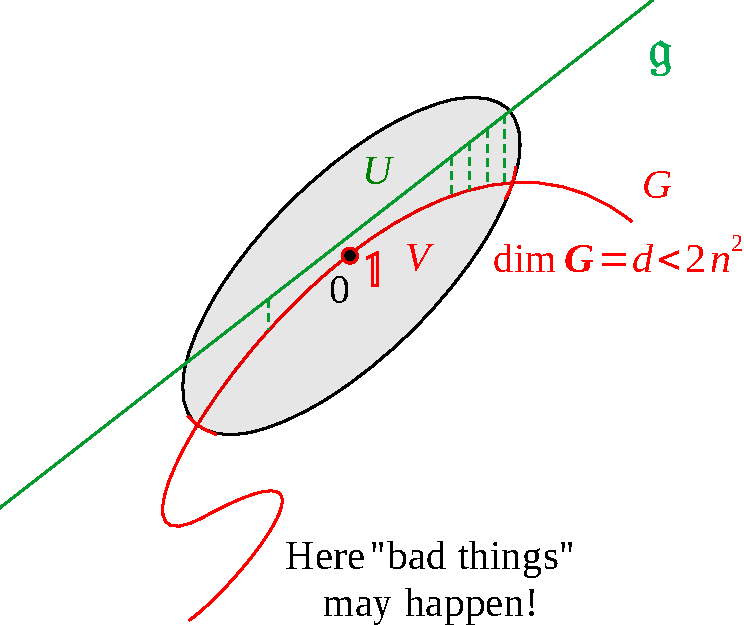
\includegraphics[width=1\linewidth]{images/visualization_exp_G2.pdf}
	\caption[Visualization of the exponential map of $G$ of the corollary]{We now added $U$ and $V$ according to the corollary for an easier identification.}
	\labfig{vis-exp-G2}
\end{marginfigure}
This justify the picture that has already many times appeared: how do we draw a Lie group in the Lie algebra?

\underline{\textbf{Visualization}:}
\begin{figure}[h!]
	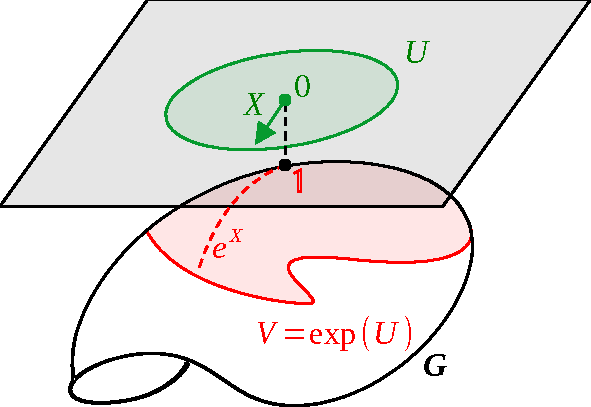
\includegraphics[width=1\linewidth]{images/visualization_corollary.pdf}
	\caption[Visualization of the corollary]{}
	\labfig{vis-corollary}
\end{figure}
The identity is the distinguish point on the Lie group $G$. Imagine to take the tangent space and to lift it. What happens is that the zero of the Lie algebra goes to the identity $\mathbb{1}$ and the vector $X$ goes down to the $e^X$. The message is that: if we take a sufficiently small ball $U$, it will be completely identified with something else, an open set (which, actually, it will be a geodesic ball) that is the image via the exponential map of $U$: $V=\exp(U)$.

Between the red set downstairs and the green set upstairs, we have a one-to-one correspondence, which moreover is $C^\infty$-smooth and with $C^\infty$-smooth inversion: a so called diffeomorphism. The main message is that if we are interested in what happens in our group, not too far from the identity (measured by the magic number), then we can simply look at the Lie algebra, that is much simpler because is a linear space. And is much simpler because the product of the group is represented locally by the brackets in the Lie algebra and the brackets are bi-linear (which is a big advantage). 

This is reason why all the people who do QM at some point leave the group and study the algebra, e.g. in the study of the representation of the rotation group: after two pages, mysteriously, we were studying the representation of the corresponding Lie algebra, as if it were the same thing.
%1:41:00
% FINE LEZIONE 19 12/05/2022
%INIZIO LEZIONE 20 13/05/2022 [scrivo tutto e poi mi sento la registrazione]
\section{Matrix $\textrm{Lie algebra}=\textrm{Lie algebra}$}
\begin{corollary}
Let G be a matrix Lie group, $\mathfrak{g}$ the \textbf{matrix} Lie algebra: 
\[
\mathfrak{g}=\{X\in\text{Mat}(n,\mathbb{C}):e^{tX}{\color{red}\in G}\quad \forall t\in\mathbb{R}\}
\]
Then, a matrix $X$ is in $\mathfrak{g}$ if and only if there exists a smooth curve 
\[
\gamma:(-\varepsilon,+\varepsilon)\xrightarrow[]{}G \ \textrm{such that}\ {\color{red}\gamma(t)\in G \ \forall t\in\mathbb{R}}, \quad\begin{cases}
\gamma(0)&=\mathbb{1}\\
\Dot{\gamma}(0)&=X
\end{cases}
\]
Thus, \[
\mathfrak{g}\cong T_eG
\]

The matrix Lie algebra is identified with the Lie algebra (as a linear space).\marginnote{We put \textit{as a linear space}, because one should still check that the Lie brackets in the matrix Lie algebra, which are just commutators of matrices, are equal to the Lie brackets geometrically defined.}
\end{corollary}
We can prove this corollary assuming the validity of the \refthm{main-exp-map}:
\begin{proof}
\underline{$\mathfrak{g}\subseteq T_eG$}: If $X\in\mathfrak{g}$, consider the path $\gamma(t)=e^{tX}$. Hence, $\gamma(t)\in G\ \forall t\in\mathbb{R}$ by definition of $G$.\sidenote{I think $\gamma(t)\in G\ \forall t\in\mathbb{R}$ \underline{by definition of $\mathfrak{g}$}, rather than "by definition of $G$".}
\[
\gamma:\mathbb{R}\xrightarrow[]{C^{\infty}}G\quad\quad\begin{cases}
\gamma(0)=e^0=\mathbb{1}\\
\Dot{\gamma}(0)=\frac{d}{dt}e^{tX}\Bigr|_{\substack{t=0}}=X
\end{cases}
\]
\underline{$T_eG\subseteq\mathfrak{g}$}: Suppose to have the following the $C^\infty$-smooth path :
\begin{align*}
    \gamma: (-\varepsilon,+\varepsilon)&\xrightarrow[]{{\color{red}C^{\infty}}}G\\
    t&\mapsto\gamma(t)
\end{align*}
so that $\gamma(0)=\mathbb{1}$ and $\Dot{\gamma}(0)=X$. We want to prove that $X\in\mathfrak{g}$.\marginnote[-15mm]{We are not asked to prove that this particular path stays in the group for every time $t$ (actually is defined only between $(\varepsilon,-\varepsilon)$ so we should find a prolungation)} As $\exp:\mathfrak{g}\xrightarrow[]{}G$ is a \textbf{local diffeomorphism} for $|t|\ll1$, therefore $\gamma(t)$ is identified with a path $\delta(t)$ in\sidenote{Il professore nei suoi appunti riporta $\delta(t)\in$ $T_eG$, ma io penso sia più corretta la versione riportata nel Capitolo 3 dell'Hall \cite{Hall2015_Ch3}.}$\mathfrak{g}$, namely,
\[
{\color{red}\gamma(t)=e^{\delta(t)}}
\]
    for some $\delta:(-\varepsilon,+\varepsilon)\to\mathfrak{g}$, with $\delta(0)=0$.\begin{marginfigure}[5mm]
    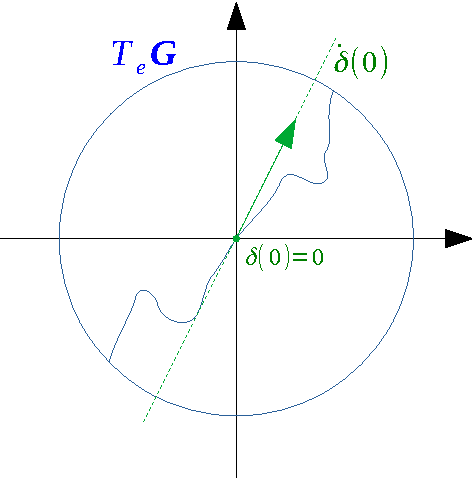
\includegraphics[]{images/lie_algebra_tangent.pdf}
    \labfig{lie_algebra_tangent}
    \caption{Scheme of $\delta(t)$ (blue line) and $t\Dot{\delta}(0)$ (dashed green line) in $T_eG$.}
\end{marginfigure} 
Notice that, as elements of the tangent space, a tangent vector is an equivalence class of paths: $[\delta(t)]=[t\Dot{\delta}(0)]$ in $T_eG$. We have to check that $\Dot{\gamma}(0)$ is in $\mathfrak{g}$:
\[
\Dot{\gamma}(0)=\dv{}{t}e^{\delta(t)}\Bigr|_{\substack{t=0}}\underset{\mathclap{\tikz \node {$\uparrow$} node [below=1ex] {\footnotesize chain rule};}}{=}\dv{}{t}e^{t\Dot{\delta}(0)}\Bigr|_{\substack{t=0}}=\Dot{\delta}(0)\,{\color{red}\stackrel{?}{\in}\mathfrak{g}} 
\]
It is, because, as we learned from Leibniz and Newton, the derivative is the limit of the incremental ratio:
\[
\Dot{\delta}(0)=\underbrace{\lim_{\varepsilon\to0}\underbrace{\frac{1}{\varepsilon}\big(\delta(\varepsilon)-\delta(0)\big)}_{\in\mathfrak{g}}}_{\in\mathfrak{g}}\in\mathfrak{g}
\]
We identified (at least at the level of vector spaces) the matrix Lie algebra and the tangent space at the identity.
\end{proof}
We should still verify that the Lie brackets agree with the commutator, then they are really isomorphic as Lie algebras and not only as vector spaces, but this is a starred exercise.

The Lie algebra captures the local structure of the Lie group (namely, the structure around the identity). We might ask ourselves, if we have two homomorphism of Lie groups, which induce the same homomorphism of the Lie algebra, will they be the same homomorphism of group?\marginnote{In a sense, the fact than they agree at the infinitesimal level, implies that they agree globally?}
\begin{corollary}
Let $G$ and H be matrix Lie groups with Lie$G=\mathfrak{g}$ and Lie$H=\mathfrak{h}$. Assume that $G$ is \textbf{connected}, and that:
\[
\begin{cases}
\Phi_1:G\xrightarrow[]{}H\\
\Phi_2:G\xrightarrow[]{}H
\end{cases} \quad \text{are Lie group homomorphisms}
\]
Let $\phi_j=\dd\Phi\Bigr|_{\substack{e}}$ be the \textbf{induced Lie algebra homomorphism}. Then, if\marginnote{Notice that the information flows from the group to the algebra. The information from the algebra to the group flows in a "not completely exact" way: we do not know what happens far away}
\[
\underset{(algebra)}{\phi_1=\phi_2}\ \Rightarrow\ \underset{(group)}{\Phi_1=\Phi_2}
\]
\end{corollary}
\section[The universal covering group ("brothers are ubiquitous")]{The universal covering group\\ ("brothers are ubiquitous")}
\underline{\textbf{Prototype:}}
\begin{enumerate}
    \item $\Phi:\textrm{SU}(2)\underset{{\color{red}\textrm{Lie}}}{\twoheadrightarrow}\textrm{SO}(3)$ is a surjective but not injective Lie group homomorphism. 
    \item At the level of the Lie algebra, it is an isomorphism $\mathfrak{su}(2)\cong\mathfrak{so}(3)$,
    \item Ker$\Phi=\{\pm\mathbb{1}\}$ is a \textbf{discrete} normal subgroup $\Rightarrow\;\textrm{SO}(3)=\textrm{SU}(2)\big/\textrm{Ker}\Phi$.
    \end{enumerate}
This behaviour is universal, up to the fact that covering is not always a two-fold covering, it could be higher.
\begin{marginfigure}
%\vspace*{-2cm}
    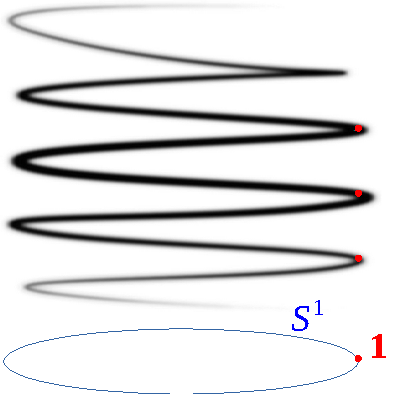
\includegraphics[]{images/spiral.pdf}
    \labfig{spiral}
    \caption*{}
\end{marginfigure} 
\begin{example}
The most basic one:
\begin{align*}
    \Phi:\mathbb{R}&\xrightarrow[]{}\text{U}(1)\\
    x&\mapsto e^{2\pi ix}
\end{align*}
$\ker\Phi=\mathbb{Z}$ and, as we know from previous courses, $\textrm{U}(1)=\mathbb{R}/2\pi\mathbb{Z}$.
\end{example}
\begin{theorem}[Universal covering]\index{Universal covering}
Let $G$ be a \underline{\textbf{connected}} Lie group. Then there exists a Lie group $\Tilde{G}$ (\textbf{unique} up to Lie group isomorphism) such that:
\begin{enumerate}
    \item Lie$G\underset{{\color{red}\text{Lie}}}{\cong}\textrm{Lie}\Tilde{G}$ (or, equivalently, G and $\Tilde{G}$ are \textbf{locally isomorphic});
    \item there exists a surjective Lie group homomorphism $\Phi:\Tilde{G}\twoheadrightarrow G$;
    \item $\Tilde{G}$ is \textbf{simply connected}.
\end{enumerate}
Moreover, $\ker\Phi\trianglelefteq\Tilde{G}$ is \textbf{discrete} and \textbf{central}, i.e. it is contained in the center of the group $Z(\Tilde{G})=\left\{h\in\Tilde{G}: hg=gh \quad \forall g\in\Tilde{G}\right\}$\marginnote{$Z$ as in \textit{zentrum} since the theory was developed by someone in Germany.}.
\end{theorem}
\begin{kaobox}[frametitle=Remark]
Given $\mathfrak{g}$, there is a unique \textbf{simply-connected Lie group} $\Tilde{G}$ such that $\textrm{Lie}\Tilde{G}=\mathfrak{g}$. All the other Lie groups with $\textrm{Lie}\textrm{G}=\mathfrak{g}$ are obtained by quotients 
\[
G=\Tilde{G}/N
\]
where $N$ is a \textbf{discrete, normal, central} subgroup of $\Tilde{G}$. 
\end{kaobox}
\end{document}